\documentclass{article}
\usepackage{tikz}

\begin{document}

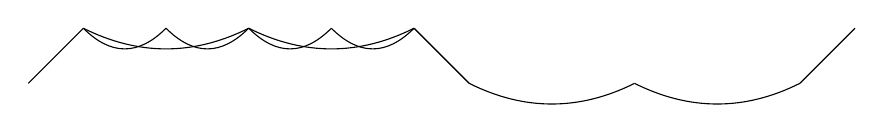
\begin{tikzpicture}[scale=0.7]
    % Draw the first part of the diagram
    \draw (0,0) -- (1,1);
    \draw (1,1) .. controls (2,0.5) and (3,0.5) .. (4,1);
    \draw (4,1) .. controls (5,0.5) and (6,0.5) .. (7,1);
    \draw (7,1) -- (8,0);
    
    % Draw the twist region
    \draw (1,1) .. controls (1.5,0.5) and (2,0.5) .. (2.5,1);
    \draw (2.5,1) .. controls (3,0.5) and (3.5,0.5) .. (4,1);
    \draw (4,1) .. controls (4.5,0.5) and (5,0.5) .. (5.5,1);
    \draw (5.5,1) .. controls (6,0.5) and (6.5,0.5) .. (7,1);
    
    % Draw the second part of the diagram
    \draw (7,1) -- (8,0);
    \draw (8,0) .. controls (9,-0.5) and (10,-0.5) .. (11,0);
    \draw (11,0) .. controls (12,-0.5) and (13,-0.5) .. (14,0);
    \draw (14,0) -- (15,1);
    
    % Add labels if needed
    % \node at (1.5,0.5) {$\cdots$};
    % \node at (11.5,0.5) {$\cdots$};
\end{tikzpicture}

\caption{Two saddle moves at the start and end of consecutive twist regions, taken from \cite[Figure 3]{BKLMR}, with crossings matching our setting.}
\label{fig:saddle_moves_twist_regions}

\end{document}